\section{Numerical radial sequence}\label{sec:sequence}
A width minimum is a numerical candidate; a resolved winding of a
specified two-component matching map adds numerical evidence; an
interval enclosure with analytic tails establishes infinite-domain
existence. Table~\ref{tab:ladder} keeps these levels separate.
The winding concept has a photonic BIC precedent~\cite{Zhen2014}; here
it is applied to a matching map in parameter space, without transferring
the photonic symmetry-based robustness theorem.
For indices 5--18, the matching map tests whether the exterior decaying
Jost solution is regular at the origin; the locations are numerical
zeros of this map. In the truncated exterior model this solution has
zero open-channel value and derivative at the outer radius and a
decaying closed-channel component. No reflecting-box eigenvalue
condition is imposed. The earlier records of indices 3--5 and the
linewidth rows 11--14 use outgoing Hankel conditions.
Increasing the outer radius by 20 and 40 units moved the locations of
indices 3, 8 and 13 by at most $1.3\times10^{-10}$ in $\omega^2$ and that
of index 18 by about $1.5\times10^{-6}$, within its estimated roundoff
level of $4.6\times10^{-6}$. This shows insensitivity to the truncation
radius, not an exact zero width.
The refined matching calculation for indices $6$--$10$ used radial
steps $0.04$ and $0.02$. Its locations interpolate parameter samples
separated by $2.5\times10^{-4}$. For indices $7$--$10$, the small
inter-grid difference ($2.3\times10^{-8}$ or less) is not a validated location error.
The reported interpolation uncertainty is a few $10^{-6}$.
For indices $11$--$14$, the archived linewidth reconstruction used signs
chosen to match neighboring slopes; index $5$ had a sign change without
a resolved winding. For this revision, indices $5$ and $11$--$14$ were
recomputed with the unchanged matching program and parameters of the
index-$15$--$18$ calculation. The rung acceptance thresholds were
retained from that calculation: one sign change of the matching error
among five starting rows, root brackets of at most $10^{-9}$ on radial
steps $0.04$ and $0.02$ with locations agreeing to $10^{-6}$, and a
rectangle crossing count $\pm1$ with alternating signs. Before this run
we additionally required a sampled phase winding equal to the crossing
count with every phase jump below $0.4$ radians. The computational time
budget was increased. The control reproduces the earlier $h=0.04$
index-$15$ root to $5\times10^{-13}$; for index $5$, the prespecified
alternation check uses index $4$. All five rungs met these conditions:
crossing counts $-1,+1,-1,+1$ for indices $11$--$14$ (and $-1$
for index $15$), $-1$ for index $5$, maximum phase jumps $0.28$--$0.30$
radians, final brackets $\le8.7\times10^{-10}$ and grid differences
$\le3.2\times10^{-8}$. The new locations differ from the earlier
estimates by $2.4\times10^{-6}$ (index $5$), $1.6\times10^{-6}$ (index
$11$) and at most $1.9\times10^{-7}$ (indices $12$--$14$). With these
locations and the subsequent index-$15$ location, the inverse-detuning
steps for indices $11$--$15$ are $2.3036$, $2.3045$, $2.3053$ and
$2.3059$. This raises the five rows to resolved numerical windings; it
is numerical evidence in the truncated model, not a certificate.

\begin{table}[htbp]\centering\small
\caption{Radial candidates at $\beta=1/2$. Displayed numerical digits
are not interval enclosures. Certificates C0/C1 are given in
Section~\ref{sec:certified-existence}; the remaining entries are finite-domain
numerical evidence. The last three error estimates are empirical.
``(0.53)'' marks rows raised by the matching calculation of this
revision.}
\label{tab:ladder}
\begin{tabular}{rll}\toprule
$n$&$\omega^2$&Evidence\\\midrule
1&$0.797676787\ldots$&Existence enclosure C0\\
2&$0.685128904\ldots$&Existence enclosure C1\\
3&$\sim0.631450$&Resolved numerical winding\\
4&$\sim0.601421$&Resolved numerical winding\\
5&$\sim0.5824198$&Resolved numerical winding (0.53)\\
6&$\sim0.569360$&Resolved numerical winding\\
7&$\sim0.559848$&Resolved numerical winding\\
8&$\sim0.552619$&Resolved numerical winding\\
9&$\sim0.546940$&Resolved numerical winding\\
10&$\sim0.542364$&Resolved numerical winding\\
11&$\sim0.5386009$&Resolved numerical winding (0.53)\\
12&$\sim0.5354487$&Resolved numerical winding (0.53)\\
13&$\sim0.5327715$&Resolved numerical winding (0.53)\\
14&$\sim0.5304696$&Resolved numerical winding (0.53)\\
15&$\sim0.52846934$&Subsequent resolved winding\\
16&$0.52671542\pm2\times10^{-7}$&Resolved winding, final bracket rule failed\\
17&$0.52516277\pm1.3\times10^{-6}$&Resolved winding, final bracket rule failed\\
18&$0.5237875\pm4\times10^{-6}$&Crossing count $+1$; phase unresolved\\\bottomrule
\end{tabular}
\end{table}

The subsequent calculation reproduced index $15$ near $0.5284693357$.
For $16$ and $17$, resolved numerical windings are $+1$ and $-1$.
For $18$, the crossing count and sampled phase winding both give $+1$,
but the maximum phase jump $0.585$ radians fails the resolution rule.
All three miss the prescribed final-bracket acceptance criterion; the
empirical errors include roundoff sensitivity. This unsuccessful
combined acceptance rule is retained, even where individual diagnostics
are informative. There is no certificate or completeness result for
these additional candidates.

\begin{figure}[htbp]\centering
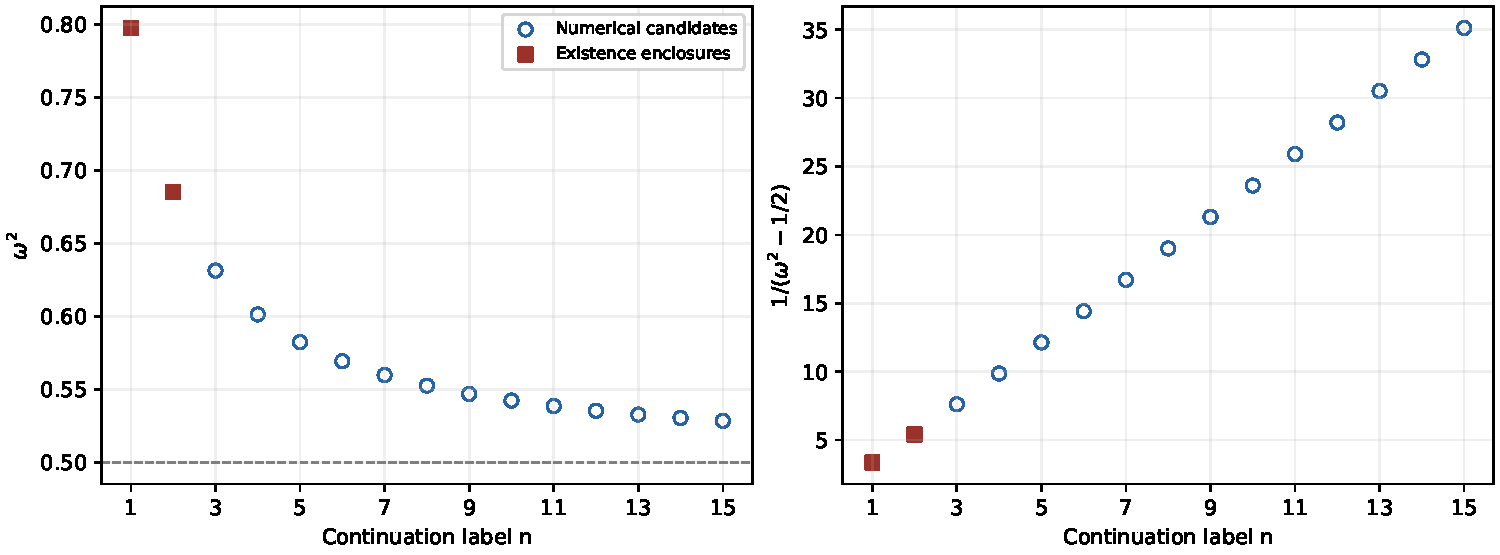
\includegraphics[width=.9\linewidth]{ladder.pdf}
\caption{Archived radial locations through $n=15$ and their inverse
detunings $1/(\omega^2-1/2)$. Filled symbols mark C0/C1. The plot retains
its original fifteen-point dataset, including the earlier rounded
index-$15$ estimate and the earlier locations of indices $5$ and
$11$--$14$; Table~\ref{tab:ladder} records the subsequent $15$--$18$
calculation and the recomputed indices $5$ and $11$--$14$ explicitly. The supplementary source inventory
binds the figure to its data. No new fit or extrapolated points are added.}
\label{fig:ladder}
\end{figure}

\paragraph{Prediction history.}\label{sec:predictions}
A sequential extrapolation was updated after each group of targets.
A separate four-parameter thin-wall fit used indices $5,7,8,9$;
its author reported separation from later target values, which were
already known to the coordination team. The frozen file of
30 September 2026, 08:33:26 CEST, and its SHA256 binding are included in
the supplementary source inventory. This is a documented calibrated
extrapolation, not global preregistration. The five later comparisons
passed their respective diagnostic windows, but showed a systematic
thin-wall offset of about $2\times10^{-5}$, comparable to those windows.
The unfitted planar comparison below therefore carries the mechanistic
interpretation; the forecast history does not establish zero linewidth.
